\section{Results}
Figure \ref{fig:Results1} shows the number of steps taken per epoch by two agents using single or team agent Q-learning for a run of 3000 epochs. Each plot shows a graph of the number of steps it takes for the agents to reach and grab the block and a graph of the number of steps it takes them to move the block to the goal. We measured the difference in performance between the two Q-learning algorithms by both speed of convergence and optimality of the learned path. 

\begin{figure}
	\centering
	\begin{subfigure}{.48\textwidth}
		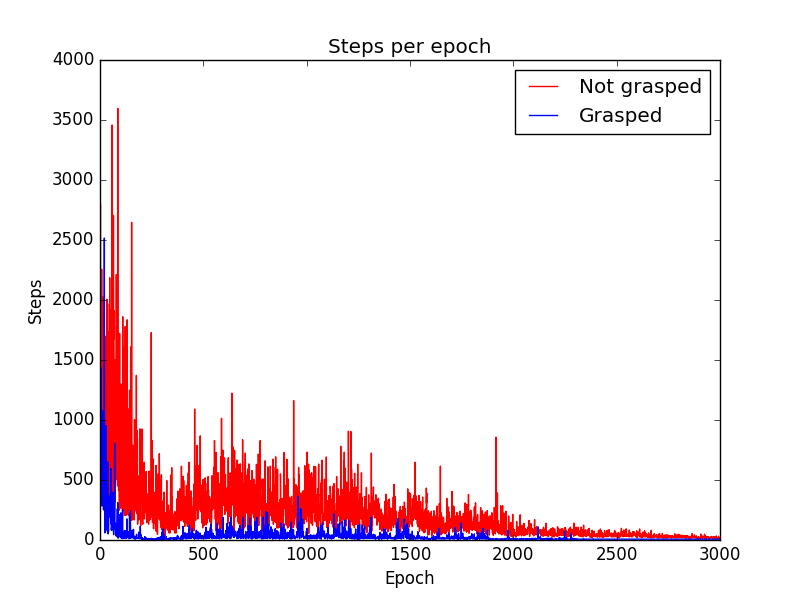
\includegraphics[width=\textwidth]{images/SingleQ.png}
		\caption{Single Q}
	\end{subfigure}
	\begin{subfigure}{0.48\textwidth}
		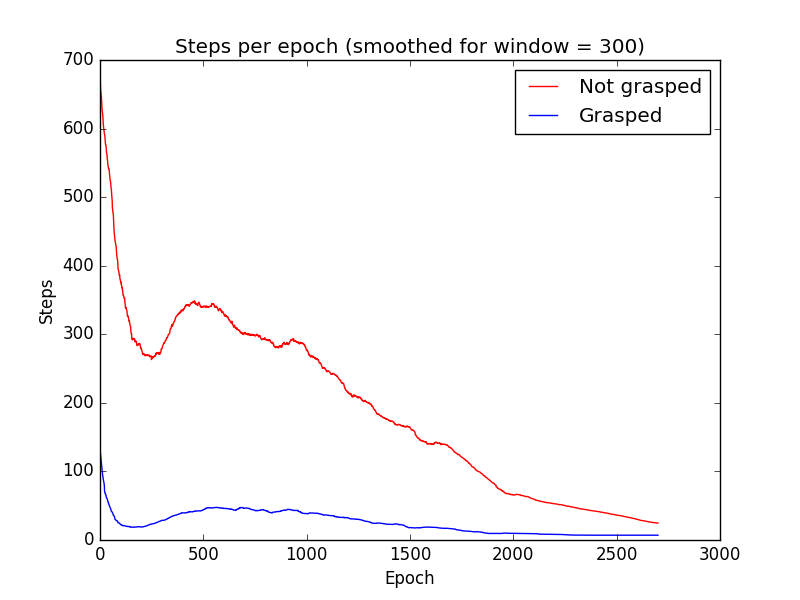
\includegraphics[width=\textwidth]{images/SingleQ_smoothed.png}
		\caption{Single Q (smoothed)}
	\end{subfigure}
	\begin{subfigure}{.48\textwidth}
		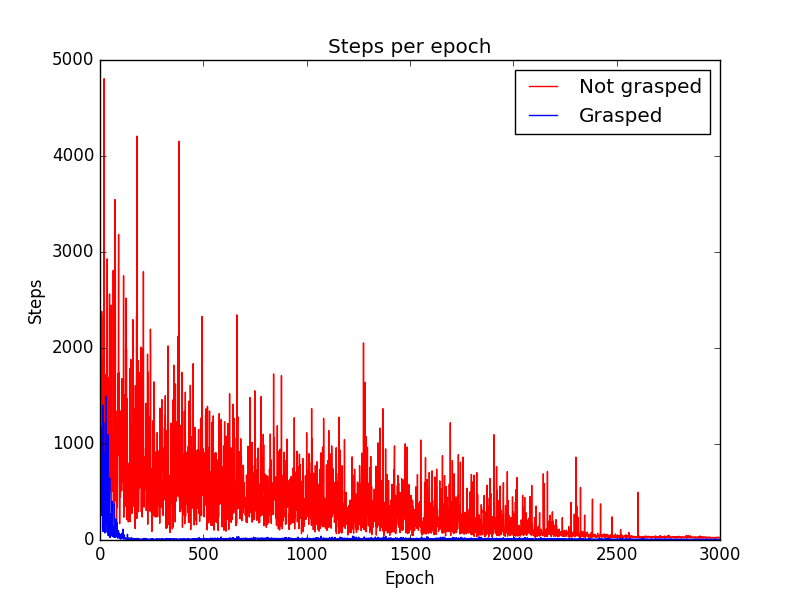
\includegraphics[width=\textwidth]{images/TeamQ.png}
		\caption{Single Q}
	\end{subfigure}
	\begin{subfigure}{0.48\textwidth}
		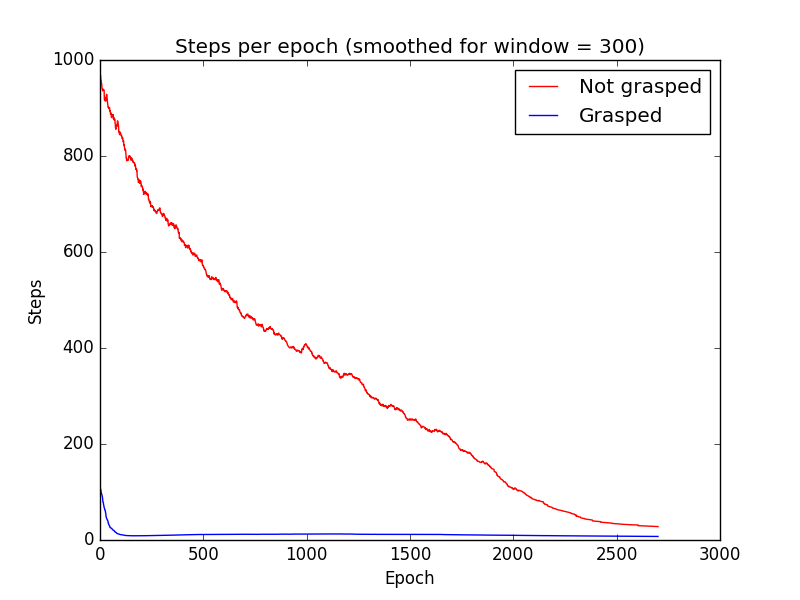
\includegraphics[width=\textwidth]{images/TeamQ_smoothed.png}
		\caption{Single Q (smoothed)}
	\end{subfigure}
	\caption{Number of steps over 3000 epochs}
	\label{fig:Results1}
\end{figure}


\subsection{Speed of convergence}
To measure the speed of convergence we used as a convergence criterion that the standard deviation of 20 consecutive epochs be smaller than a set value.\footnote{For these results $\sigma_{not_grabbed} < 7$ and $\sigma_{grabbed} < 2$}. Figures \ref{3a} and \ref{3b} show the standard deviations for both the single and team learning algorithm. The simulation was run 30 times per learning algorithm and every run the number of epochs it took to reach the convergence criterion was counted. Figures \ref{3c} and \ref{3d} show the results of these counts.

To test whether the difference was significant we performed an unpaired t-test on the not grabbed, grabbed and summed results. The t-test tested highly significant for the not grabbed samples with $m_{single} = 2636.6$ and $m_{team} = 2500.0$: $t(55.331) = 3.8914$, $p < 0.001$. It also tested highly significant for the grabbed samples, with $m_{single} = 1776.767$ and $m_{team} = 205.9$: $t(29.279) = 35.443$, $p<0.001$. Finally, the t-test tested highly significant for the added results, with $m_{single} = 4413.367$ and $m_{team} = 2705.9$: $t(44.634) = 36.169$, $p < 0.001$. 
\begin{figure}
	\centering
	\begin{subfigure}{.48\textwidth}
		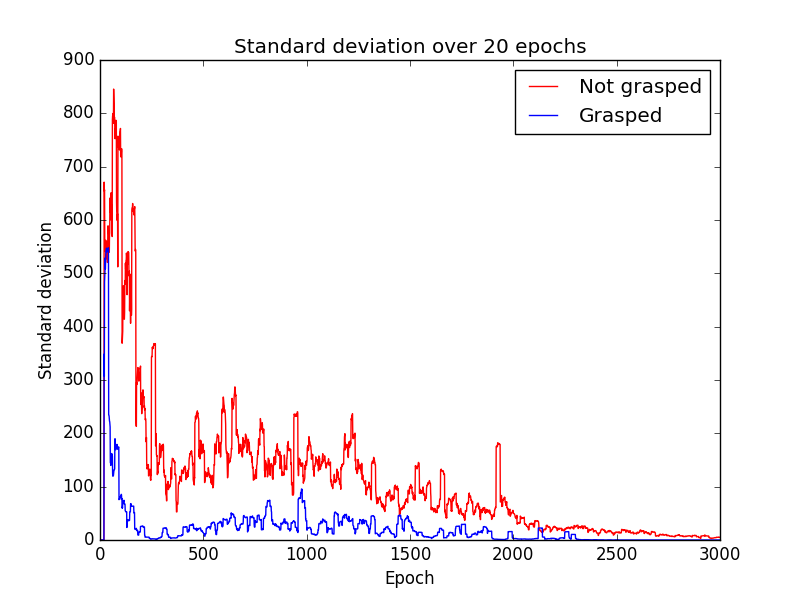
\includegraphics[width=\textwidth]{images/Stdev_single.png}
		\caption{Single Q}
		\label{3a}
	\end{subfigure}
	\begin{subfigure}{0.48\textwidth}
		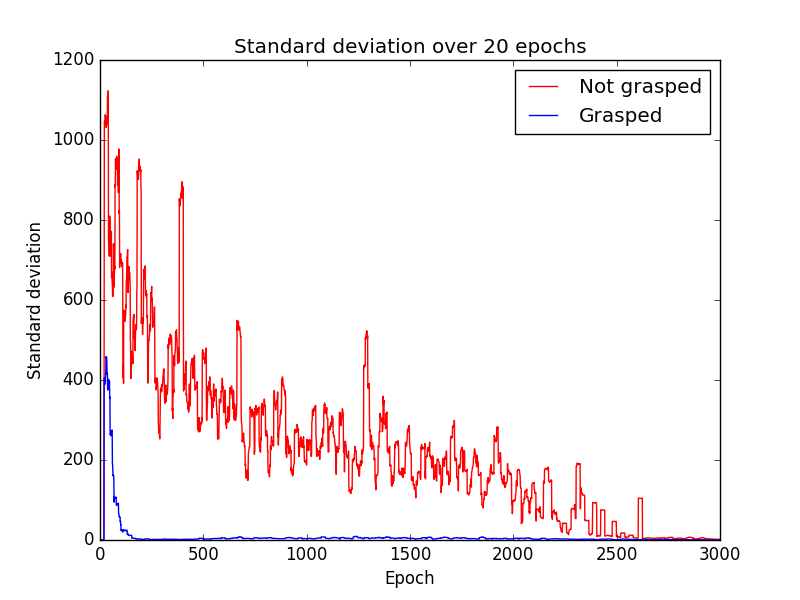
\includegraphics[width=\textwidth]{images/Stdev_team.png}
		\caption{Team Q}
		\label{3b}		
	\end{subfigure}
	\begin{subfigure}{.48\textwidth}
		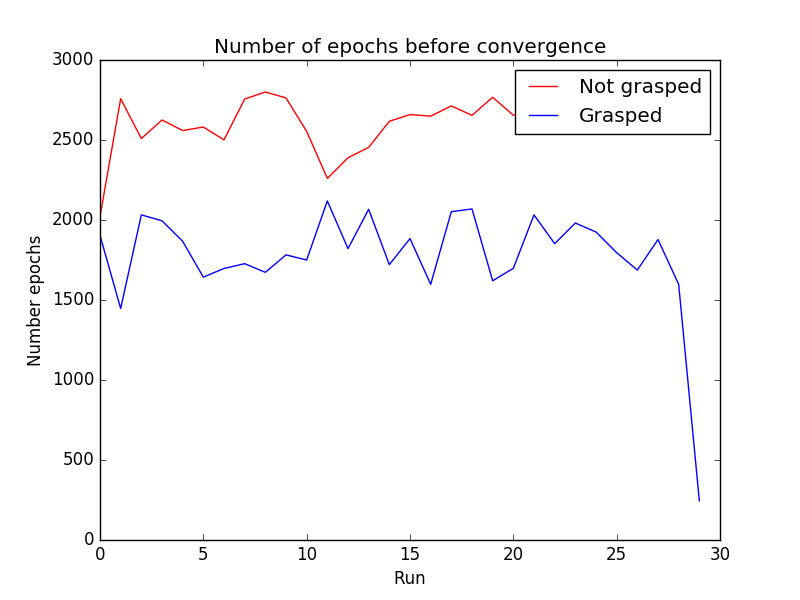
\includegraphics[width=\textwidth]{images/Convergence_single.png}
		\caption{Single Q}
		\label{3c}		
	\end{subfigure}
	\begin{subfigure}{0.48\textwidth}
		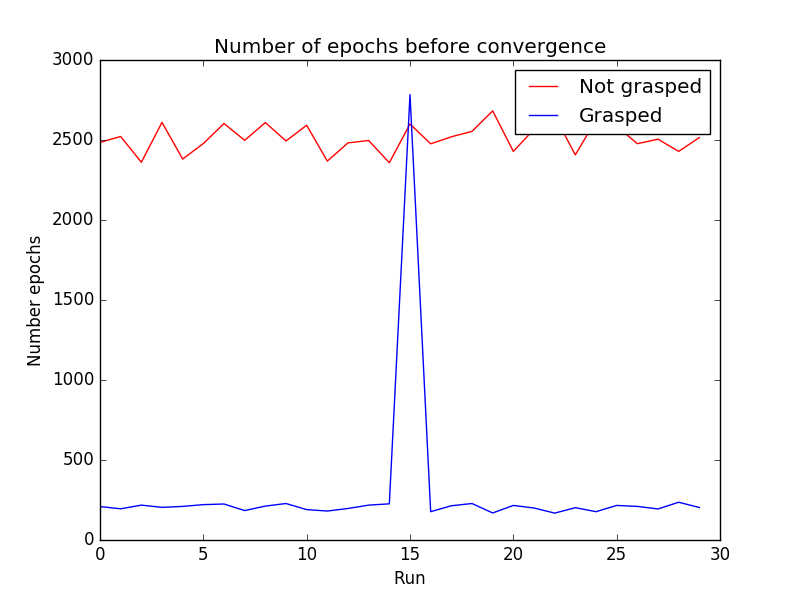
\includegraphics[width=\textwidth]{images/Convergence_team.png}
		\caption{Team Q}
		\label{3d}		
	\end{subfigure}
	\caption{(a and b) Standard deviation over 20 epochs in a run of 3000 epochs. (c and d) Epochs before convergence.}
	\label{fig:Results3}
\end{figure}

From these results we can conclude that single Q-learning is converged slightly faster when the block is not grabbed, but considerably slower when the block is grabbed. In total this results in the team Q-learning being quite faster overall, with an average difference of approximately 1707 epochs. Note that this difference is taken over the sum of the epochs for grabbed and not grabbed samples. Since the algorithms do both the grabbed and not grabbed part during one epoch, you might also consider just the difference between the samples with the highest number of epochs, which in both cases is the not grabbed one. This difference was still measured highly significant, but is much smaller: ca. 137 epochs.